\documentclass[11pt]{beamer}

%%%%%%%% tema e cor %%%%%%%%
\mode<presentation> {
\usetheme{Madrid}
%\usecolortheme{albatross}
}
\usepackage{amsmath}
\usepackage{hyperref}

%\usepackage[brazil]{babel}
\usepackage[utf8]{inputenc}
\usepackage{graphicx} 
\usepackage{booktabs} 



{
%================= logos no meio =====================

%\medskip
%\texttt{\{lods.eng,ronety\}@uea.edu.br} % emails
}
\date{\today}

\AtBeginSection[]
{
\begin{frame}
\frametitle{Outline}
\tableofcontents[currentsection]
\end{frame}
}

%%%%%%%% titulo e subtitulo %%%%%%%%
\title[Policy Gradient Methods]{Policy Gradient Methods in Reinforcement Learning} 

%%%%%%%% nome dos autores %%%%%%%%
\author[Kabir Ahuja]{
Kabir Ahuja} 

\begin{document}
\begin{frame}
\titlepage 

\end{frame}

\begin{frame}
\frametitle{Outline} 
\tableofcontents 
\end{frame}

%%%%%%%% slides %%%%%%%%
\section{Introduction} 
\begin{frame}{The Reinforcement Learning Problem}
\begin{columns}
\column{0.5\textwidth}
\begin{itemize}
\item Deals with agents learning to take decisions in an environment that provides numerical rewards.
\item The goal of the agent is to maximize the cumulative reward obtained by interacting with environment
\end{itemize}

\column{0.5\textwidth}
\centering
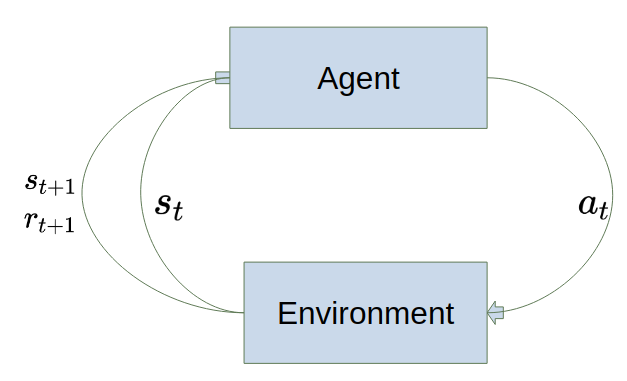
\includegraphics[scale = 0.25]{img/block.png}
\end{columns}
\end{frame}
\begin{frame}{Markov Decision Process (MDP)}
\begin{itemize}
    \item Mathematical Formulation of RL problem.
    \item Based on the \textbf{Markov property} which means that the current state completely captures the state of the world. More concretely:
    $P(s_{t+1}|s_t)$ = $P(s_{t+1}|s_t, s_{t-1}, ..., s_0)$ \item Defined by $(S, A, \mathbb{R},  \mathbb{P}, \gamma)$ 
    \begin{itemize}
        \item $S$ : set of possible states
        \item $A$ : set of possible actions
        \item $\mathbb{R}$ : distribution of reward given (state, action) pair. 
        \item $\mathbb{P}$ : transition probability which gives the distribution of next state given a (state, action) pair. 
        \item $\gamma$ : discount factor
    \end{itemize}
\end{itemize}
    
\end{frame}
\begin{frame}{Policy}
\begin{itemize}
    \item A policy describes the behavior of an agent.
    \item It is a function that maps state to action.
    \item Deterministic Policy:
        $a_t = \pi(s_t; \theta)$
    \item Stochastic Policy:
        $a_t \sim \pi(a_t|s_t;\theta)$
    \item The goal of an RL agent is to learn a policy which maximizes the agent’s cumulative discounted reward (also called return) which is defined as: $\sum_{t > 0}\gamma^{t-1}r_t$
\end{itemize}
\end{frame}
\begin{frame}{Value Functions} 
\begin{columns}
\column {0.5\textwidth}
\centering
\textbf{State Value Function}
\begin{itemize}
    \item A value function describes how good or bad a particular \textbf{state} is.
    \item It is defined by the expected cumulative reward starting from state $s_t$ and following a policy $\pi$.
    \newline
    $V_{\pi}(s_t) = \mathop{\mathbb{E}}_{\pi}[r_t + \gamma r_{t+1} + ... + \gamma^{T-t}r_{T} | s_t]$
    \item The optimal value function is defined as the maximum value function for all the policies.
    $V(s_t) = max_{\pi}(V_{\pi}(s_t))$
\end{itemize}
\column {0.5\textwidth}
\centering
\textbf{Action Value Function}
\begin{itemize}
    \item Describes how good a \textbf{state, action} pair is.
    \item It is defined as the expected cumulative reward obtained on starting from a state $s_t$, taking action $a_t$ and then following a policy $\pi$
    \newline
    $Q_{\pi}[s_t,a_t] =\mathop{\mathbb{E}}_{\pi}[r_t + \gamma r_{t+1} + ... + \gamma^{T-t}r_{T} | s_t, a_t] $
    \item The optimal Q value function can be defined as the maximum of q value functions for all the policies.
    $Q(s_t, a_t) = max_{\pi}(Q_{\pi}(s_t, a_t))$
\end{itemize}
\end{columns}
    
\end{frame}
\begin{frame}{Solving the RL Problem}
\begin{itemize}
    \item Value based RL
    \begin{itemize}
        \item Learn optimal action value function $Q$
        \item Policy is the generated implicitly from the learned $Q$ function (greedy, $\epsilon$ greedy)
        \item Eg: Q Learning, SARSA, Monte Carlo Control etc.
    \end{itemize}
    \item Policy based RL (Policy Gradient Methods)
    \begin{itemize}
        \item Learn the policy $\pi$ directly.
        \item Eg: REINFORCE , A2C, TRPO, PPO, DDPG etc.   
    \end{itemize}
\end{itemize}
    
\end{frame}


\section{Policy Based RL}
\begin{frame}{Parameterized Policies}
\begin{itemize}
    \item For the purpose of this lecture we will focus on policies parameterized by Neural Nets.
    \item For \textbf{Discrete action spaces}, the network takes the state representation as the input and outputs the probabilities of taking each action (Softmax Policy). Analogus to classification in Supervised Learning.
\end{itemize}
\begin{center}
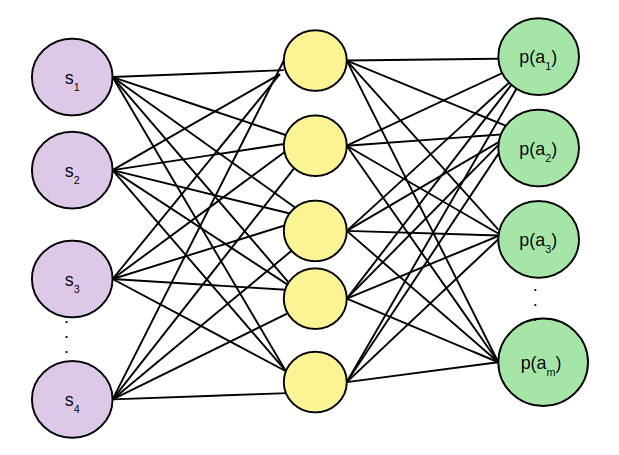
\includegraphics[scale=0.3]{img/discaction.png}
\end{center}
\end{frame}
\begin{frame}{Parameterized Policies}
\begin{itemize}
    \item In case of \textbf{Continuous action spaces}, we assume our policy to be gaussian and the network takes the state as input and outputs the mean and diagonal covariance of the distribution. Analogus to regression in Supervised Learning.
\end{itemize}
\begin{center}
    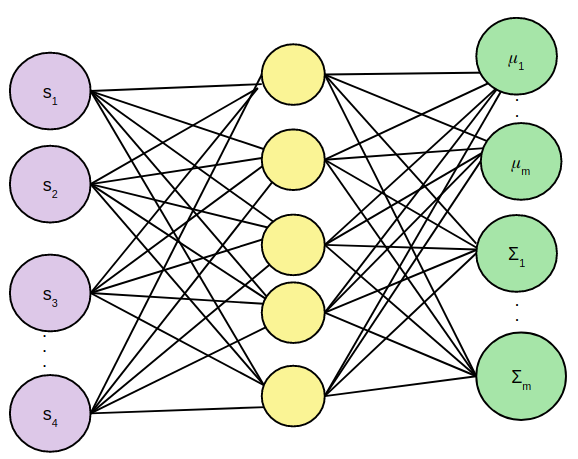
\includegraphics[scale=0.3]{img/contaction.png}

\end{center}
\end{frame}
\begin{frame}{Policy Optimization Objective}
\begin{columns}
\column{0.45\textwidth}
    \begin{itemize}
        \item[] $s_0 \sim \mu(s_0)$
        \item[] $a_0 \sim \pi(a_0|s_0;\theta)$
        \item[] $s_1 \sim \mathbb{P}(s_1|s_0, a_0)$
        \item[] $r_0 \sim \mathbb{R}(s_0, a_0, s_1)$
        \item[] $a_1 \sim \pi(a_1|s_1;\theta)$
        \item[] $s_2 \sim \mathbb{P}(s_2|s_1, a_1)$
        \item[] $r_1 \sim \mathbb{R}(s_1, a_1, s_2)$
        \item[] ...
        \item[] $a_{T-1} \sim \pi(a_{T-1}|s_{T-1};\theta)$
        \item[] $s_T \sim \mathbb{P}(s_T|s_{T-1}, a_{T-1})$
        \item[] $r_{T-1} \sim \mathbb{R}(s_{T-1}, a_{T-1}, s_{T})$
    \end{itemize}
\column{0.55\textwidth}
    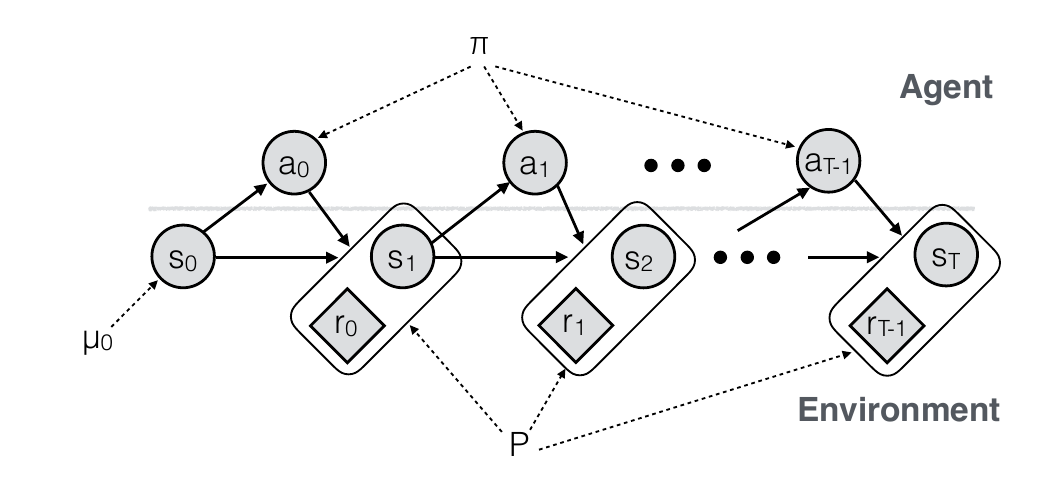
\includegraphics[scale=0.18]{img/trajvis.png}
\end{columns}
\footnotetext[1]{Image from John Schulman slides on Policy Gradients.}
\end{frame}
\begin{frame}{Policy Optimization Objective}
\textbf{Objective Function}
\newline
maximize $\eta(\pi_{\theta})$
\newline
where
\begin{equation}
    \begin{split}
        \eta(\pi_{\theta}) & = \mathop{\mathbb{E}_{\tau}}[r_0 + \gamma r_1 + \gamma^2 r_2 + ... + \gamma^{T-1}r_{T-1}|\pi_{\theta}]\\
        & = \mathop{\mathbb{E}_{\tau}}[R(\tau)|\pi_{\theta}]
    \end{split}
\end{equation}
and $\tau$ denotes a trajectory $(s_0,a_0,r_0,s_1,a_1,r_1,...,s_T, a_{T-1}, r_{T-1})$
\newline
\textbf{Intuition}
\newline
By maximizing this objective function we:
\begin{itemize}
    \item Make the good trajectories more probable.
    \item By making good trajectories more probable we also make good actions more probable.
\end{itemize}
\end{frame}
\begin{frame}{Solving the Optimization Problem}
\begin{itemize}
    \item Note that our objective function is not a direct function of policy parameters $\theta$
    \item To optimize the function using gradient based methods we need a way to estimate the gradients of the objective with respect to $\theta$
    \item \textbf{Score function gradient estimator}  is used for this purpose.
\end{itemize}
    
\end{frame}

\begin{frame}{Score Function Gradient Estimator}
\begin{itemize}
    \item Consider an optimization problem of maximizing $\mathop{\mathbb{E}}_{x \sim p(x|\theta)}[f(x)]$ with respect to $\theta$
\end{itemize}
\begin{equation}
    \begin{split}
            \nabla_{\theta}\mathop{\mathbb{E}_x}[f(x)] & = \nabla_{\theta} \sum_x p(x|\theta)f(x)\\
    & = \sum_x \nabla_{\theta}p(x|\theta)f(x)\\
    & = \sum_x p(x|\theta)\frac{\nabla_{\theta}p(x|\theta)}{p(x|\theta)}f(x)\\
    & = \sum_x p(x|\theta)\nabla_{\theta}\log p(x|\theta)f(x)\\
    & = \mathop{\mathbb{E}_x}[f(x) \nabla_{\theta}\log p(x|\theta)]\\
    \end{split}
\end{equation}
    
\end{frame}
\begin{frame}{Score Function Gradient Estimator}
\textbf{Intuition}
\newline 
Lets denote the score function estimator as $g_i = f(x_i)\nabla_{\theta} \log p(x_i|\theta)$
\begin{itemize}
    \item Let $f(x)$ denotes how good a sample $x$ is.
    \item Moving in the direction of $g$ pushes the probability of $x$ in the proportion of how good it is ($f(x)$).
    \item A sample which leads to a small value of $f(x)$ will lead to adjustment of parameters $\theta$ such that its log probability is reduced as compared to the samples with higher $f(x)$ and vice versa.
    \item  \textbf{$f(x)$ need not be a continuous or differentiable function}.
\end{itemize}
    
\end{frame}
\begin{frame}{Score Function Gradient Estimator}
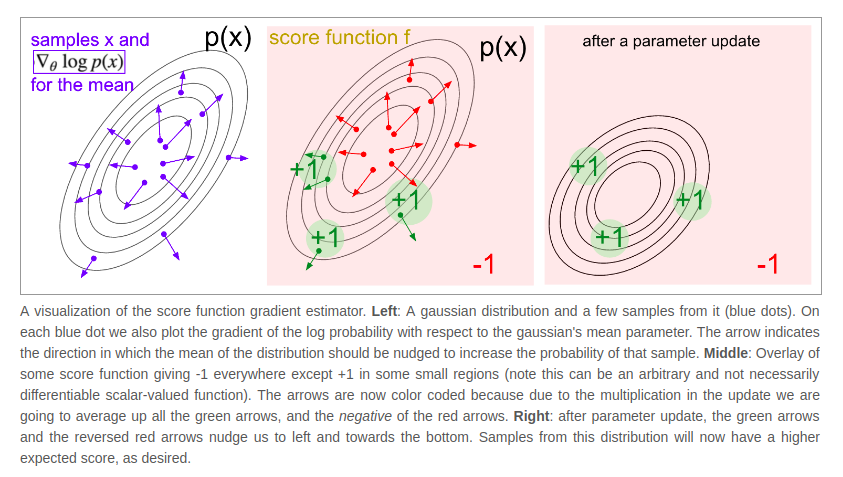
\includegraphics[scale = 0.4]{img/scoreFunction.png}
 \footnotetext[1]{Image from Andrej Karpathy's blog\\ (https://karpathy.github.io/2016/05/31/rl/)}
\end{frame}
\begin{frame}{Score Function Gradient Estimator for Policies}
\begin{itemize}
    \item Remember our objective function was: $\max_{\theta}$ $\mathop{\mathbb{E}_{\tau}}[R(\tau)]$
    \item The random variable $x$ in this case is the trajectory $\tau$ denoted by $(s_0,a_0,r_0,s_1,a_1,r_1,...,s_T, a_{T-1}, r_{T-1})$
    \item And the function $f$ is the total cumulative reward. $f(\tau) = R(\tau) = \sum_t \gamma^tr_t$
    \item The probability of the trajectory can be computed as:
\end{itemize}
\begin{equation*}
    \begin{split}
        &p(\tau) = \mu(s_0)\pi(a_0|s_0;\theta)\mathbb{P}(s_1|s_0,a_0)\pi(a_1|s_1;\theta)\mathbb{P}(s_2|s_1,a_1)...\\
        &p(\tau)= \mu(s_0)\prod_{t=0}^{T-1} \pi(a_t|s_t;\theta)\mathbb{P}(s_{t+1}|s_t,a_t)\\
    &\log p(\tau) = \log \mu(s_0) + \sum_{t=0}^{T-1}\log\pi(a_t|s_t;\theta) + \sum_{t=0}^{T-1}\log \mathbb{P}(s_{t+1}|s_t,a_t)
    \end{split}
\end{equation*}

    
\end{frame}
\begin{frame}{Score Function Gradient Estimator for Policies}
    \begin{equation*}
        \begin{split}
            & \nabla_\theta \log p(\tau) = \nabla_\theta \sum_{t=0}^{T-1}\log\pi(a_t|s_t;\theta) \\
            & \nabla_\theta \mathop{\mathbb{E}_\tau}[R] = \mathop{\mathbb{E}_\tau}[R \nabla_\theta \sum_{t=0}^{T-1}\log\pi(a_t|s_t;\theta)]\\
            & \nabla_\theta \mathop{\mathbb{E}_\tau}[R] = \mathop{\mathbb{E}_\tau}[(\sum_{t=0}^{T-1} \gamma^tr_t)( \nabla_\theta \sum_{t=0}^{T-1}\log\pi(a_t|s_t;\theta))]
        \end{split}
    \end{equation*}
    \textbf{Intuition}: Good trajectories i.e. the trajectories with higher values of $R$ will serve as supervised examples like in the case of classification or regression.
\end{frame}

\begin{frame}{Score Function Gradient Estimator for Policies}
    \begin{itemize}
        \item A slightly better estimate can be obtained by rearranging the terms in the expression above and we obtain:
        $\nabla_\theta \mathop{\mathbb{E}_\tau}[R] = \mathop{\mathbb{E}_\tau}[ \nabla_\theta \sum_{t=0}^{T-1}\log\pi(a_t|s_t;\theta)\sum_{t' = t}^{T-1} \gamma^{t'} r_{t'}]$
        \item The second term in the expression can be interpreted as an estimate of action value function (Q)
        $\nabla_\theta \mathop{\mathbb{E}_\tau}[R] = \mathop{\mathbb{E}_\tau}[\nabla_\theta \sum_{t=0}^{T-1}\log\pi(a_t|s_t;\theta)Q(s_t,a_t)]$
    \end{itemize}
\end{frame}
\begin{frame}{Practical Implementation with Autodiff}
\begin{itemize}
    \item Collect $n$ different trajectories $\tau_i = (s_0^i,a_0^i,r_0^i,s_1^i,a_1^i,r_1^i,...,s_T^i, a_{T-1}^i, r_{T-1}^i)$
    \item For each trajectory $\tau_i$ compute Q value estimates
    $Q(s_t^i, a_t^i) = \sum_{t' = t}^{T-1}\gamma^{t'}r_{t'}^i$
    \item The log probabilities can be obtained from the output of neural network $f$.
    \begin{itemize}
        \item For Discrete Action Spaces:
        $\log\pi(a_t^i|s_t^i;\theta) = \log f(s_t^i;\theta)$
        \item For Continuous Action Spaces:
        \begin{equation*}
            \begin{split}
               &\mu_t^i, \sigma_t^i = f(s_t;\theta)\\
                &\log\pi(a_t^i|s_t^i;\theta) = \frac{-(a_t^i-\mu_t^i)^2}{2\sigma_t^{i2}} - \frac{1}{2}\log(2\pi^k\sigma_t^i)
            \end{split}
        \end{equation*}
    \end{itemize}
\end{itemize}

\end{frame}
\begin{frame}{Practical Implementation with Autodiff}
    \begin{itemize}
    \item Define the surrogate loss as:
    $L_{surr}(\theta) = -\frac{\sum_{i = 1}^n \sum_{t=0}^{T-1}Q(s_t^i,a_t^i)\log\pi(a_t|s_t;\theta))}{n}$
    \item Find policy gradient estimate: $g(\theta) = \nabla_{\theta}L_{surr}(\theta)$
    \begin{itemize}
        \item Pytorch: loss.backward()
        \item Tensorflow : tf.train.Optimizer().minimize(loss)
    \end{itemize}
    \item Plug $g(\theta)$ in your favourite optimizer SGD/ ADAM
    \item This algorithm is called REINFORCE or Vanilla Policy Gradient
\end{itemize}
\end{frame}
\begin{frame}{Collecting Trajectories}
    \begin{itemize}
        \item[] Initialize sets $S, A, R, P$ for storing states, actions, rewards and neural network outputs.
        \item[] Sample initial state $s_0$ from environment $E$
        \item[] t = 0
        \item[] \textbf{Repeat} till episode \textbf{terminates}
        \begin{itemize}
            \item[] Sample action $a_t$ from $\pi(a_t|s_t,\theta)$ defined using the outputs of neural network $f(s_t)$. (Multinomial Distribution for discrete case and Gaussian for continuous)
            \item[] Execute action $a_t$ in environment $E$ and obtain reward $r_t$ and new state $s_{t+1}$
            \item[] Store $s_t, a_t, r_t, f(s_t)$ in the sets $S, A, R, P$
            \item[] t := t+1
        \end{itemize}
    \end{itemize}
\end{frame}
\begin{frame}{REINFORCE Algorithm}
    \begin{itemize}
        \item[] Initialize policy parameters $\theta$
        \item[] \textbf{for} iteration = 1,2... \textbf{do} 
        \begin{itemize}
            \item[] Collect a set of trajectories using current policy $\pi$.
            \item[] At each time step for each trajectory compute the approximate Q value as: $Q(s_t^i, a_t^i) = \sum_{t' = t}^{T-1}\gamma^{t'}r_{t'}^i$
            \item[] Compute the log probabilities $\log\pi(a_t|s_t;\theta)$ using the output of the neural net.
            \item[] Compute the surrogate loss using log probabilities and Q values.
            \item[] Compute the gradient $g(\theta)$  of the loss function and update the parameters of policy: For eg. SGD Update: $\theta = \theta - \alpha g(\theta)$
        \end{itemize}
        \item[] \textbf{end for}
    \end{itemize}
\end{frame}


\section{Non Differentiable Computation in Neural Nets}
\begin{frame}{Upside of Policy Gradients}
\begin{columns}
\column {0.55\textwidth}
\begin{itemize}
    \item One of the most attractive thing about policy gradients is that the reward function need not be differentiable with respect to the policy parameters.
    \item This provides us with a framework to handle non differentiable computation when working with neural networks.
    \item Such situation often arises when we require sampling from a probability distribution during the forward pass or when we require to optimize a non differentiable objective function. 
\end{itemize}
\column {0.45\textwidth}
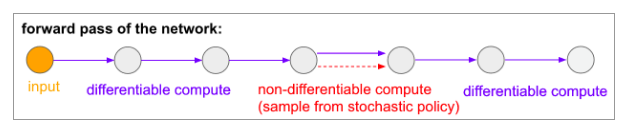
\includegraphics[scale = 0.25]{img/nondiffcomput.png}
\newline
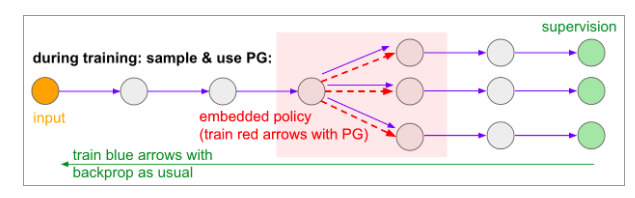
\includegraphics[scale = 0.25]{img/nondiffcomput2.png}
\end{columns}
  \footnotetext[1]{Image from Andrej Karpathy's blog\\ (https://karpathy.github.io/2016/05/31/rl/)}
\end{frame}
\begin{frame}{Case Study: Optimizing BLEU for NMT}
    \begin{itemize}
        \item For training Machine Translation systems we optimize the negative log likelihood of the predictions of decoder.
        \item However NLL loss might not be the best measure of the quality of translation.
        \item For evaluation of the translation by an NMT model we often use metrics like BLEU.
        \item However using standard supervised learning approaches we can not directly optimize BLEU since it requires the access to the predicted tokens, not the probabilities.
        \item To make matters worse BLEU calculation is non differentiable so even if we manage to select the tokens by a differentiable operation (max pool) it will still be problematic.
    \end{itemize}
\end{frame}
\begin{frame}{Case Study: Optimizing BLEU for NMT}
    \begin{itemize}
        \item Policy Gradients to the rescue!
        \item We can represent the machine translation problem as an MDP:
            \begin{itemize}
                \item State $s_t$ : The state at time step $t$ will be given by the input token to the decoder at time $t$ and the hidden state of the decoder $h_t$ which encompasses information from the previous time steps of decoder as well as the hidden states of encoder.
                \item Action $a_t$ : The action at time step $t$ is given by the prediction of decoder at time $t$. This hence becomes a case of discrete action space and we can use a softmax policy.
                \item Reward $r_t$: We use a delayed reward in this case where 0 reward is given at all time steps and at final step reward equal to the BLEU score between the prediction and the ground truth is used.
                \item Transition $\mathbb{P}$ : Transition in this case will be given by the input token at the next time step and the updated hidden state of RNN $h_t$
            \end{itemize}
    \end{itemize}
\end{frame}

\begin{frame}{Case Study: Optimizing BLEU for NMT}
    \begin{itemize}
        \item Now we can simply use the REINFORCE algorithm to train our translation system.
        \item Please note that the action space for this problem is quite large (equal to the number of words in the vocabulary).
        \item Directly training the model with REINFORCE will be very slow and might not even converge to a good policy.
        \item People often first train their model using the standard supervised learning approach and then fine tune it using policy gradients.
    \end{itemize}
\end{frame}

\section{Limitations of Policy Gradients}
\begin{frame}{Downside of Policy Gradients}
Vanilla Policy Gradients suffers from 2 serious problems:
\begin{itemize}
    \item High variance of gradient estimates
    \item Highly sample inefficient
\end{itemize}
\end{frame}

\begin{frame}{High Variance of gradient estimates}
    \begin{columns}
        \column {0.6\textwidth}
        \begin{itemize}
            \item As we saw before the policy gradient is given by: $\nabla_\theta \mathop{\mathbb{E}_\tau}[R] = \mathop{\mathbb{E}_\tau}[ \nabla_\theta \sum_{t=0}^{T-1}\log\pi(a_t|s_t;\theta)\sum_{t' = t}^{T-1} \gamma^{t'} r_{t'}]$
            \item However during implementation we estimate this expectation using only a few examples which leads to a very high variance in the estimate, especially for long trajectories and high dimensional action spaces.
            \item One natural way of reducing variance is to collect a lot of trajectories before calculating the policy gradient.
        \end{itemize}
        \column{0.4\textwidth}
        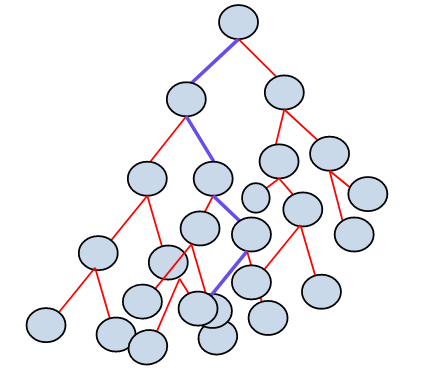
\includegraphics[scale = 0.3]{img/highvar.png}
    \end{columns}
\end{frame}
\begin{frame}{High Variance of gradient estimates}
    \begin{columns}
        \column {0.6\textwidth}
        \begin{itemize}
            \item Using discount factor also reduces the variance to an extent since it diminishes the importance of future rewards.
            \item However these 2 tricks are not always sufficient to solve the problem.
            \item One way of reducing variance which is mostly used in practice is by subtracting the Q value estimate with an appropriate baseline.
            \item Actor critic methods (A2C, A3C) learn a baseline to reduce the variance. (Will be discussed in next tutorial)
        \end{itemize}
        \column{0.4\textwidth}
        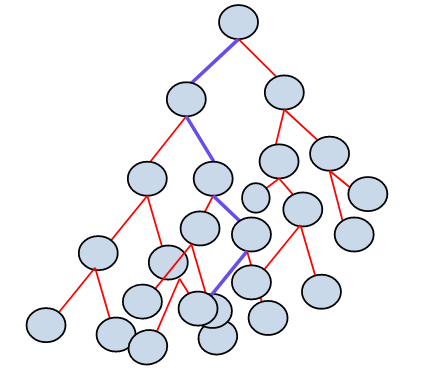
\includegraphics[scale = 0.3]{img/highvar.png}
    \end{columns}    
\end{frame}

\begin{frame}{Sample Efficiency}
    \begin{columns}
        \column{0.5\textwidth}
        \begin{itemize}
            \item The vanilla policy gradient algorithm has a very bad sample efficiency.
            \item The collected trajectories can only be used for a single gradient update.
            \item After making the update we throw away the data that was collected and collect new experience using the updated policy for the next update.
            \item In many cases collecting data might be very expensive (for eg. In Robotics)
        \end{itemize}
        \column{0.5\textwidth}
        
\includegraphics[scale = 0.35]{img/thanos.png}
    \end{columns}
\end{frame}
\begin{frame}{Sample Efficiency}
\begin{itemize}
    \item To better understand why this problem occurs, lets look again at the equation of policy gradients: $\nabla_\theta \mathop{\mathbb{E}_\tau}[R] = \mathop{\mathbb{E}_\tau}[ \nabla_\theta \sum_{t=0}^{T-1}\log\pi(a_t|s_t;\theta)\sum_{t' = t}^{T-1} \gamma^{t'} r_{t'}]$
    \item The expectation is over the trajectory distribution which is a function of policy. 
    \item Once we update the policy, the trajectory distribution will change too.
    \item Hence the collected samples will no longer be valid to compute this expectation.
    \item Variants of vanilla policy gradients like TRPO, PPO (next tutorial) modify the policy gradient to enable multiple policy updates using the collected samples.
    \item Off policy variants like DDPG enables the use of experience replay which helps in using the samples from past experience to make policy updates.
\end{itemize}
\end{frame}

%%%%%%%% agradecimentos %%%%%%%%

%------------------------------------------------


%------------------------------------------------
%------------------------------------------------
%%%%%%%% referencias %%%%%%%%
\nocite{*}
\begin{frame}{References}
\begin{enumerate}
    \item John Schulman's slides on Policy Gradients: \href{http://rail.eecs.berkeley.edu/deeprlcoursesp17/docs/lec2.pdf}{http://rail.eecs.berkeley.edu/deeprlcoursesp17/docs/lec2.pdf}
    \item David Silver's slides on Policy Gradients: \href{http://www0.cs.ucl.ac.uk/staff/d.silver/web/Teaching_files/pg.pdf}{http://www0.cs.ucl.ac.uk/staff/d.silver/web/Teaching\_files/pg.pdf}
    \item Andrej Karpathy's Blog on Policy Gradients: \href{https://karpathy.github.io/2016/05/31/rl/}{https://karpathy.github.io/2016/05/31/rl/}
    \item Lijun Wu, Fei Tian, Tao Qin, Jianhuang Lai, Tie-Yan Liu: "A Study of Reinforcement Learning for Neural Machine Translation" (2018)
\end{enumerate}
\end{frame}

\begin{frame}{}
\begin{center}
\Huge Thank you!
\end{center}
\end{frame}


\end{document}